% Ejercicio 3 (1): grafica de f(x,y) = x^3 + 6x^2 + 3y^2 - 12xy + 9x.
% Como f(x,y) = 3(y-2x)^2 + x(x-3)^2, la grafica es un valle a lo largo de
% la recta y = 2x. Se dibuja sobre la franja {(x, 2x+w) : 0 <= x <= 4.2,
% |w| <= 1.3}. Los puntos marcados son la silla (1,2,4) y el minimo local (3,6,0).
\documentclass[tikz,border=3pt]{standalone}
\usepackage{pgfplots}
\pgfplotsset{compat=1.18}
\begin{document}
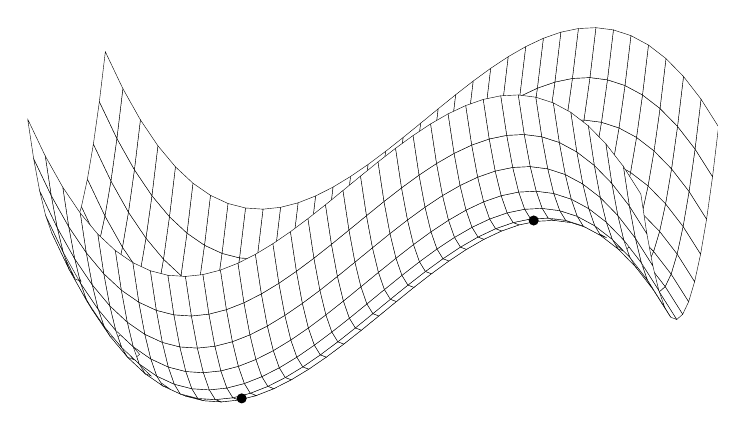
\begin{tikzpicture}
  \begin{axis}[
      hide axis,
      view={-150}{30},
      width=20cm, height=16cm,
      unit vector ratio*=1 1 0.6,
      domain=0:4.2, y domain=-1.3:1.3,
      samples=36, samples y=14,
      z buffer=sort,
    ]
    \addplot3[surf, shader=faceted, faceted color=black, fill=white,
      opacity=1, line width=0.15pt, mesh/ordering=y varies]
      ({x},{2*x+y},{3*y^2+x*(x-3)^2});
    \addplot3[only marks, mark=*, mark size=1.6pt, black]
      coordinates {(1,2,4) (3,6,0)};
  \end{axis}
\end{tikzpicture}
\end{document}
